

\chapter{Design Concept} \label{chapter:desgin}

\section{Design concept with JQuery Mobile Framework}
In this chapter it will be explained how the project NAVAR used the jQuery Mobile Framework,CSS3 and HTML5 to create the user Interface of the APP NAVAR. This chapter will describe how to use  the components of the JQuery mobile framework. The reason why the project NAVAR uses Javascript,HTML5,
CSS3 and jQuery Mobile for the user interface is, that the design can be used for other platforms. This pictures shows how the app is built:
\\\\
\begin{figure}[htbp]
\centering
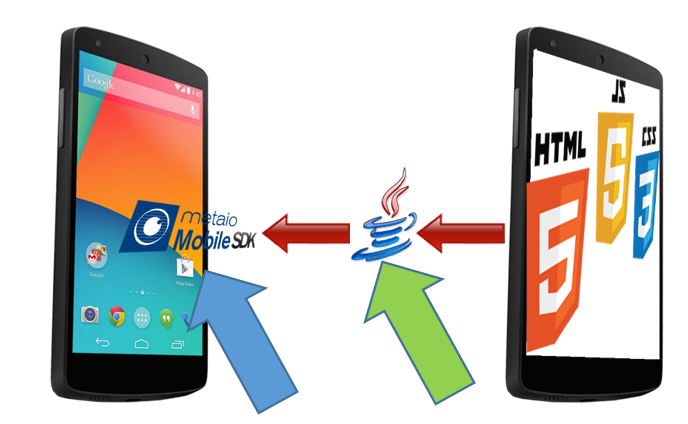
\includegraphics[width=240pt,height=180pt,keepaspectratio]{graphics/AppStructure.PNG}
\end{figure}
\\\\
The blue arrow shows the SDK of Metaio. The Metaio SDK will be explained in the chapter Implementation. Moreover, if Metaio GmbH creates a SDK for another platform, so it should be necessary to change the SDK and Java Components of this project NAVAR(green arrow). NAVAR was built with modularity. There is then no need to change something in the user interface because it can be used for every mobile platform.
\\\\

\subsubsection{jQuery Mobile Page}
The Basic of jQuery Mobile is to create a blank page and then to define the components such as Button or Listview, etc, which defines the interaction for the user interface.  The blank page is a HTML File. It has the same basic html tag structure. The main benefit of the jQuery Mobile Framework is, there are attributes for each component or HTML tag such as:
\\
\begin{itemize}
\item data-theme $\rightarrow$ to Define the colour of a component
\item data-role $\rightarrow$ defines the components in HTML such as Button,Listview or Link
\item data-icon $\rightarrow$  defines which icon should be used for the HTML component.
\end{itemize}

There are more data- attributes which are defined in this jQuery Mobile API:  http://demos.jquerymobile.com/1.2.0/docs/api/data-attributes.html\\\\     
\newpage The following Codesnippet will show  the Source Code looks for a jQuery Mobile page:

\begin{lstlisting}[language=html,caption= jQuery Page,captionpos=b]
<html>
<head>
    <title>NAV-AR</title>
    <link href="css/jquery.mobile-1.3.2.min.css" 
    rel="stylesheet" type="text/css"/>
    <script src="js/jquery-1.9.1.min.js" 
    type="text/javascript">
    </script>
    <script src="js/jquery.mobile-1.3.2.min.js" 
    type="text/javascript">
    </script>
    <script type="text/javascript" src="js/notifier.js">
    </script>    
<body>
<div data-role="header">
</div>
<div data-theme="a" data-role="footer" 
data-position="fixed" data-id="footer">
    <a class="ui-btn-left" href="index.html" 
    rel="external">Back</a>
</div>
</body>
</html>

\end{lstlisting}

Listing 2.1 shows how to add the Library into a HTML and how to create Header, Footer from jQuery Mobile Framework. Furthermore how to use the data-role Attribute, it is often defined in HTML container Tag called div.\\\\

\subsubsection{Mainmenu}
In this segment it will be explained how to use the Listview to create a Menu with navigation form. The usage of Lists are for data display, navigation, result lists, and data entry. First of all ,to create a  Listview, the html file have to include jQuery Mobile library$\rightarrow$Code:
\begin{lstlisting}[language=html,caption= Input Library,captionpos=b]
<script src="js/jquery.mobile-1.3.2.min.js"
 type="text/javascript"></script>

\end{lstlisting}

It is possible to create a dynamical Listview, but for the dynamic function it needs JavaScript. For the menu of the APP the list view is static. This Figure shows the syntax for the Listview:

\begin{figure}[htbp]
\centering
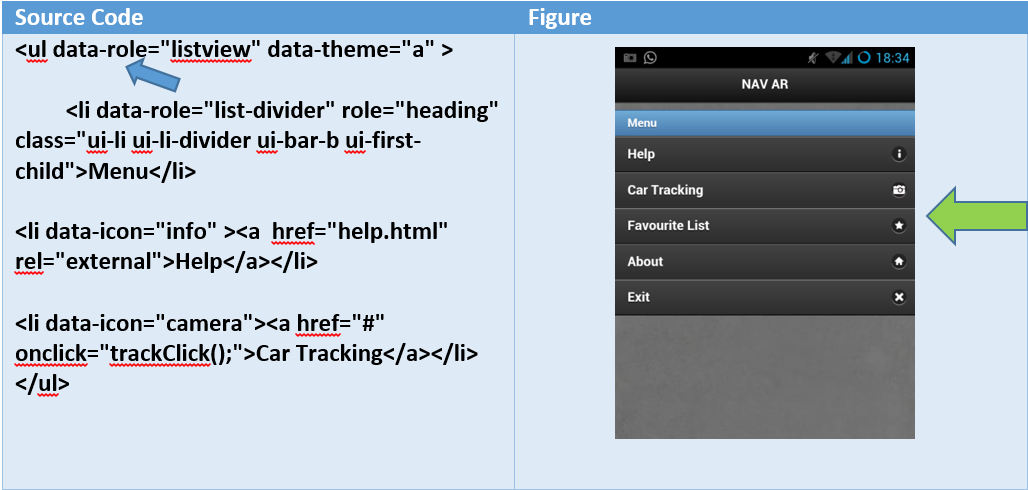
\includegraphics[width=1.0\linewidth]{graphics/Menu.PNG}
\caption{Menu Page}
\end{figure}

Jquery Mobile uses the HTMLTags  to create a component of  jQuery mobile and to define the data-role. Data-role is an attribute which can be used if the JQuery Mobile Library is included(Blue arrow). For this project the List items(Green Arrow) are linked to another html Files or it invokes a Function.\\\\
\newpage
\subsubsection{Slide Panel}
The Slide Panel is one of the big functionalities of the jQuery Mobile Framework. With the Slide Panel it is possible to make it easy to create menus, collapsible columns, drawers, inspectors panes and more. The Panel have to be defined in a jQuery Mobile Page. Furthermore the Panel can not be placed outside of the page. The Figure shows ,how the panel looks like with the code snippet of this project NAVAR. The main point is to a create panel and to define the attribute data-role to a panel(Blue arrow.)\\\\
Afterwards the project has List Items in the panel for a menu. The user can navigate easily through the user interface with this feature.\cite{Panel}


\begin{figure}[h]
\centering
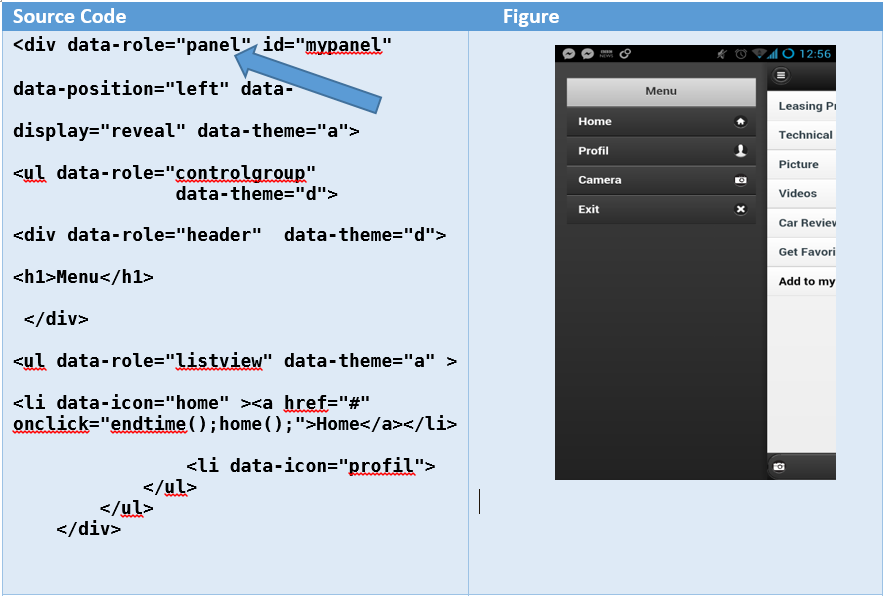
\includegraphics[width=1.0\linewidth]{graphics/SPanel.PNG}
\caption{Slide Panel}
\end{figure}
\clearpage

The Panel has to defined in the header of jQuery Mobile page or as Button function. This  code snippet  shows how to do it. First all the Panel has to been defined with a id to get reference of it.
Codesnippet:
\begin{lstlisting}[language=html,caption= Panel definition in Header,captionpos=b]
<div data-role="header">
        <h1>NAV AR</h1>

         <a href="#mypanel" data- 
          icon="bars" data- 
        iconpos="notext">Menu</a>

    </div>
s
\end{lstlisting}
\subsubsection{jQuery Mobile Table}
JQuery Mobile Framework has the feature to create a table. In this project tables are very important, because the Information from the Navision Server will be list in a table. The following code snippet will show how it works :
\begin{figure}[H]
\centering
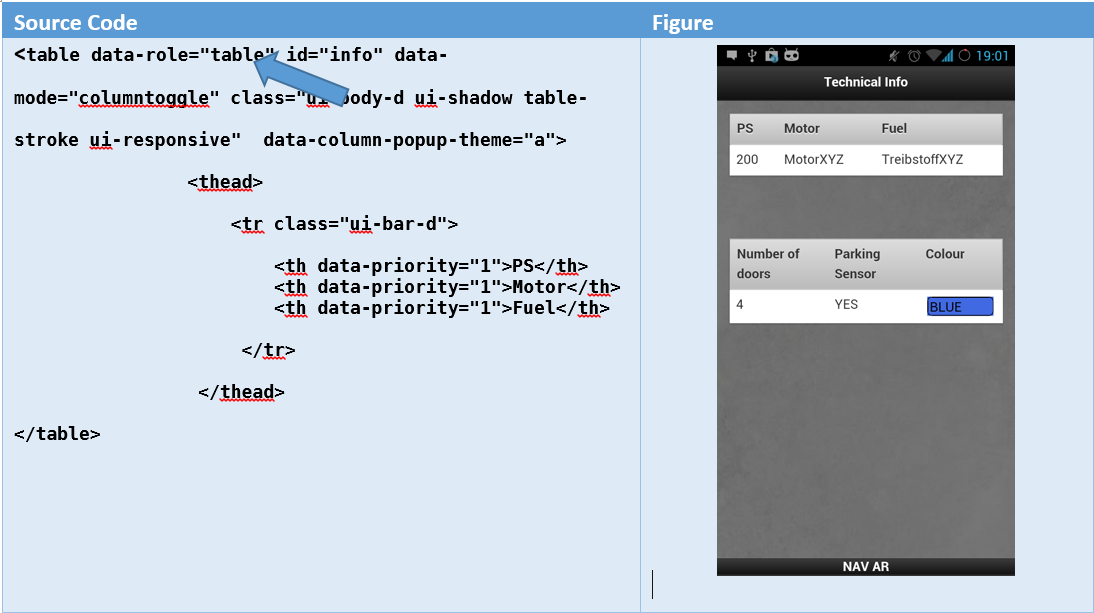
\includegraphics[width=1.0\linewidth]{graphics/Table.PNG}
\caption{Table}
\end{figure}
shows the attribute data-role should have bee defined as 'table'(Blue Arrow).With the other attributes such as:
Data--mode, data--column--popup--theme. With these attributes it is possible to define the appearance of the table.

\newpage
\section{Video Gallery}
The video Gallery in our mobile-application gives the user the possibility to watch test reviews and commercial videos of the tracked car.
\\

   
For implementing the YouTube car video gallery we used \textbf{jquery} and the jquery plug-in \textbf{jquery.youtubevideogallery}. The Design and CSS files were taken from Jack Moore's plug-ins. \cite{jqueryVideo}. His great work makes it possible to dynamically scale the size and position of the video-boxes so that they perfectly fit on every device screen! 
\\

As one can see in the figure on the next page the position and size automatically adjust to the 3 different screen sizes.    

\begin{figure}[H]
\centering
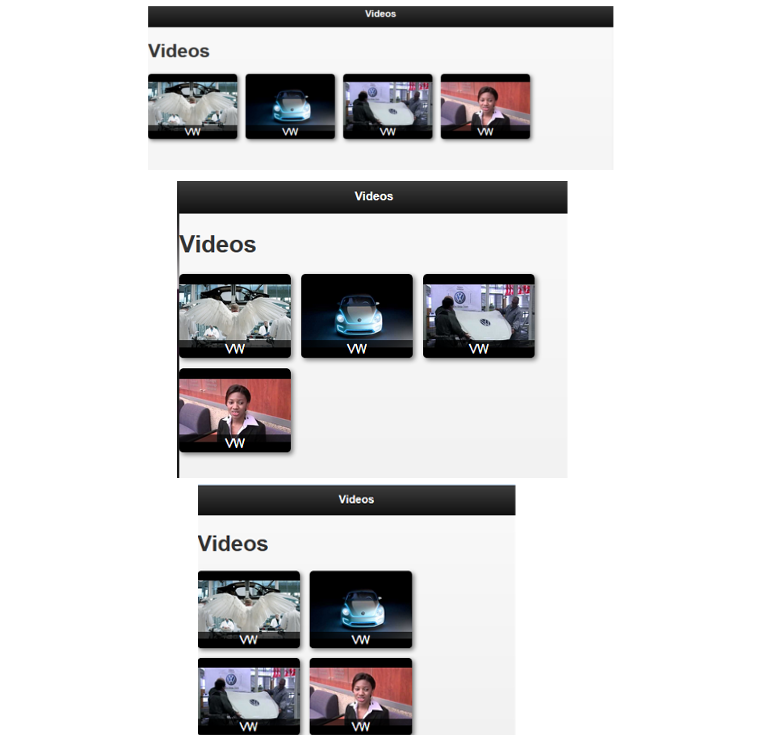
\includegraphics[width=\textwidth,height=\textheight,keepaspectratio]{graphics/dynamic.png}
\caption{dynamically fit to device screen}
\end{figure}  

\newpage
\subsection{Implementation}
We wrote a JavaScript script that appends an array of different YoutTube video url to an \textbf{ul} tag which uses the \textbf{youtube-videogallery} class.   
\begin{lstlisting}[language=html, caption= 
extracts from the video gallery src,captionpos=b]
<ul id="Gallery" class="youtube-videogallery">
	<script>
	... 
	//append video urls
	for (var i=0; i<videos.length; i++){
		$("#Gallery").append(videos[i]);
	}
	</script>
</ul>
<!-- Use jack Mores .js for the gallery -->
<script>
    $(document).ready(function(){
        $("ul.youtube-videogallery").
        youtubeVideoGallery( 
        {plugin:'colorbox',assetFolder:'../'} );
    });
</script> 
\end{lstlisting}
